\documentclass[11pt,aspectratio=169]{beamer}
% =============================================================================
%  Shared Beamer preamble — Machine Learning I & II, PEU-CD 2026 (ENEI / INEI)
%
%  Inherited from the ML_Foundations deck (Alexander Quispe), with three changes:
%    * `minted` removed — it shells out to Pygments and does not build under
%      tectonic; every code block in the course uses `listings`.
%    * unused packages (lipsum, blindtext, multimedia, videoframe) dropped.
%    * `bbm` dropped — its fonts are PK-only and tectonic cannot render them;
%      the indicator uses \mathbf{1} instead.
%    * a math-macro block added so all twelve lectures share one notation.
%
%  Each lecture is a standalone document:
%      \documentclass[11pt,aspectratio=169]{beamer}
%      % =============================================================================
%  Shared Beamer preamble — Machine Learning I & II, PEU-CD 2026 (ENEI / INEI)
%
%  Inherited from the ML_Foundations deck (Alexander Quispe), with three changes:
%    * `minted` removed — it shells out to Pygments and does not build under
%      tectonic; every code block in the course uses `listings`.
%    * unused packages (lipsum, blindtext, multimedia, videoframe) dropped.
%    * `bbm` dropped — its fonts are PK-only and tectonic cannot render them;
%      the indicator uses \mathbf{1} instead.
%    * a math-macro block added so all twelve lectures share one notation.
%
%  Each lecture is a standalone document:
%      \documentclass[11pt,aspectratio=169]{beamer}
%      % =============================================================================
%  Shared Beamer preamble — Machine Learning I & II, PEU-CD 2026 (ENEI / INEI)
%
%  Inherited from the ML_Foundations deck (Alexander Quispe), with three changes:
%    * `minted` removed — it shells out to Pygments and does not build under
%      tectonic; every code block in the course uses `listings`.
%    * unused packages (lipsum, blindtext, multimedia, videoframe) dropped.
%    * `bbm` dropped — its fonts are PK-only and tectonic cannot render them;
%      the indicator uses \mathbf{1} instead.
%    * a math-macro block added so all twelve lectures share one notation.
%
%  Each lecture is a standalone document:
%      \documentclass[11pt,aspectratio=169]{beamer}
%      \input{../../../style/preamble}
% =============================================================================

% ---------- fonts ----------
\usepackage{helvet}
\usepackage[default]{lato}
\usepackage{tgbonum}
\usepackage{mathpazo}
\usepackage[utf8]{inputenc}

% ---------- math ----------
\usepackage{amsmath,amssymb}
\usepackage{mathtools}

% ---------- graphics, tables, layout ----------
\usepackage{graphicx}
\usepackage{tikz}
\usetikzlibrary{positioning,calc,arrows,arrows.meta,decorations.markings,shapes.misc,matrix,shapes,fit}
\usepackage{array}
\usepackage{booktabs}
\usepackage{multirow}
\usepackage{dcolumn}
\usepackage{subcaption}
\usepackage{caption}
\usepackage{changepage}
\usepackage{xspace}
\usepackage{tcolorbox}
\tcbuselibrary{skins,breakable}
\usepackage[ruled,vlined]{algorithm2e}
\usepackage{listings}
\usepackage{appendixnumberbeamer}
\usepackage{hyperref}

\newcolumntype{d}[0]{D{.}{.}{5}}
\setbeamertemplate{caption}[numbered]

% ---------- palette (Okabe–Ito, colour-blind safe) ----------
\definecolor{blue}{RGB}{0,114,178}
\definecolor{red}{RGB}{213,94,0}
\definecolor{yellow}{RGB}{240,228,66}
\definecolor{green}{RGB}{0,158,115}
\definecolor{MyBackground}{RGB}{255,253,218}

\hypersetup{colorlinks=true, linkbordercolor={white}, linkcolor={blue}, urlcolor={blue}}

% ---------- beamer look ----------
\setbeamercolor{frametitle}{fg=blue}
\setbeamercolor{title}{fg=black}
\setbeamertemplate{footline}[frame number]
\setbeamertemplate{navigation symbols}{}
\setbeamertemplate{itemize items}{-}
\setbeamercolor{itemize item}{fg=blue}
\setbeamercolor{itemize subitem}{fg=blue}
\setbeamercolor{enumerate item}{fg=blue}
\setbeamercolor{enumerate subitem}{fg=blue}
\setbeamercolor{button}{bg=MyBackground,fg=blue}
\setbeamercolor{section in toc}{fg=blue}
\setbeamercolor{subsection in toc}{fg=red}
\setbeamersize{text margin left=1em,text margin right=1em}
\setbeamercolor{block title}{fg=white,bg=blue}
\setbeamercolor{block body}{bg=blue!5}
\setbeamercolor{block title alerted}{fg=white,bg=red}
\setbeamercolor{block body alerted}{bg=red!5}
\setbeamercolor{block title example}{fg=white,bg=green}
\setbeamercolor{block body example}{bg=green!5}
\setbeamertemplate{blocks}[rounded][shadow=false]

\newenvironment{wideitemize}{\itemize\addtolength{\itemsep}{10pt}}{\enditemize}

\newenvironment{transitionframe}{
  \setbeamercolor{background canvas}{bg=yellow}
  \begin{frame}}{
  \end{frame}
}

% Section divider: a plain frame with a large blue title.
\newcommand{\sectionframe}[1]{%
  \section{#1}%
  \begin{frame}[plain]\vfill\begin{center}{\Huge\textcolor{blue}{#1}}\end{center}\vfill\end{frame}}

% ---------- proof / derivation environments ----------
% derivation: a boxed, step-by-step algebraic argument. Title is the claim.
\newtcolorbox{derivation}[1]{enhanced, colback=blue!3, colframe=blue, fonttitle=\bfseries,
  title={#1}, boxrule=0.6pt, left=4pt, right=4pt, top=3pt, bottom=3pt, arc=2pt}
% claim: a result to be proved (theorem / lemma / proposition).
\newtcolorbox{claim}[1]{enhanced, colback=white, colframe=black, fonttitle=\bfseries,
  title={#1}, boxrule=0.6pt, left=4pt, right=4pt, top=3pt, bottom=3pt, arc=2pt}
% keypoint: the one line to remember from a slide.
\newtcolorbox{keypoint}{enhanced, colback=green!6, colframe=green, boxrule=0.6pt,
  left=4pt, right=4pt, top=3pt, bottom=3pt, arc=2pt}
% caution: a common mistake or a subtlety.
\newtcolorbox{caution}{enhanced, colback=red!5, colframe=red, boxrule=0.6pt,
  left=4pt, right=4pt, top=3pt, bottom=3pt, arc=2pt}

% ---------- code ----------
\lstset{
  basicstyle=\ttfamily\scriptsize, keywordstyle=\color{blue}\bfseries,
  commentstyle=\color{green}, stringstyle=\color{red},
  showstringspaces=false, breaklines=true, frame=single, rulecolor=\color{black!30},
  numbers=none, xleftmargin=4pt, framexleftmargin=4pt, language=Python
}

\input{../../../style/macros}

% ---------- course-wide title metadata ----------
\newcommand{\courseinstitution}{ENEI -- INEI \,\textperiodcentered\, PEU-CD 2026}
\newcommand{\courseauthor}{Alexander Quispe}
\institute{\courseinstitution}
\author{\courseauthor}

% =============================================================================

% ---------- fonts ----------
\usepackage{helvet}
\usepackage[default]{lato}
\usepackage{tgbonum}
\usepackage{mathpazo}
\usepackage[utf8]{inputenc}

% ---------- math ----------
\usepackage{amsmath,amssymb}
\usepackage{mathtools}

% ---------- graphics, tables, layout ----------
\usepackage{graphicx}
\usepackage{tikz}
\usetikzlibrary{positioning,calc,arrows,arrows.meta,decorations.markings,shapes.misc,matrix,shapes,fit}
\usepackage{array}
\usepackage{booktabs}
\usepackage{multirow}
\usepackage{dcolumn}
\usepackage{subcaption}
\usepackage{caption}
\usepackage{changepage}
\usepackage{xspace}
\usepackage{tcolorbox}
\tcbuselibrary{skins,breakable}
\usepackage[ruled,vlined]{algorithm2e}
\usepackage{listings}
\usepackage{appendixnumberbeamer}
\usepackage{hyperref}

\newcolumntype{d}[0]{D{.}{.}{5}}
\setbeamertemplate{caption}[numbered]

% ---------- palette (Okabe–Ito, colour-blind safe) ----------
\definecolor{blue}{RGB}{0,114,178}
\definecolor{red}{RGB}{213,94,0}
\definecolor{yellow}{RGB}{240,228,66}
\definecolor{green}{RGB}{0,158,115}
\definecolor{MyBackground}{RGB}{255,253,218}

\hypersetup{colorlinks=true, linkbordercolor={white}, linkcolor={blue}, urlcolor={blue}}

% ---------- beamer look ----------
\setbeamercolor{frametitle}{fg=blue}
\setbeamercolor{title}{fg=black}
\setbeamertemplate{footline}[frame number]
\setbeamertemplate{navigation symbols}{}
\setbeamertemplate{itemize items}{-}
\setbeamercolor{itemize item}{fg=blue}
\setbeamercolor{itemize subitem}{fg=blue}
\setbeamercolor{enumerate item}{fg=blue}
\setbeamercolor{enumerate subitem}{fg=blue}
\setbeamercolor{button}{bg=MyBackground,fg=blue}
\setbeamercolor{section in toc}{fg=blue}
\setbeamercolor{subsection in toc}{fg=red}
\setbeamersize{text margin left=1em,text margin right=1em}
\setbeamercolor{block title}{fg=white,bg=blue}
\setbeamercolor{block body}{bg=blue!5}
\setbeamercolor{block title alerted}{fg=white,bg=red}
\setbeamercolor{block body alerted}{bg=red!5}
\setbeamercolor{block title example}{fg=white,bg=green}
\setbeamercolor{block body example}{bg=green!5}
\setbeamertemplate{blocks}[rounded][shadow=false]

\newenvironment{wideitemize}{\itemize\addtolength{\itemsep}{10pt}}{\enditemize}

\newenvironment{transitionframe}{
  \setbeamercolor{background canvas}{bg=yellow}
  \begin{frame}}{
  \end{frame}
}

% Section divider: a plain frame with a large blue title.
\newcommand{\sectionframe}[1]{%
  \section{#1}%
  \begin{frame}[plain]\vfill\begin{center}{\Huge\textcolor{blue}{#1}}\end{center}\vfill\end{frame}}

% ---------- proof / derivation environments ----------
% derivation: a boxed, step-by-step algebraic argument. Title is the claim.
\newtcolorbox{derivation}[1]{enhanced, colback=blue!3, colframe=blue, fonttitle=\bfseries,
  title={#1}, boxrule=0.6pt, left=4pt, right=4pt, top=3pt, bottom=3pt, arc=2pt}
% claim: a result to be proved (theorem / lemma / proposition).
\newtcolorbox{claim}[1]{enhanced, colback=white, colframe=black, fonttitle=\bfseries,
  title={#1}, boxrule=0.6pt, left=4pt, right=4pt, top=3pt, bottom=3pt, arc=2pt}
% keypoint: the one line to remember from a slide.
\newtcolorbox{keypoint}{enhanced, colback=green!6, colframe=green, boxrule=0.6pt,
  left=4pt, right=4pt, top=3pt, bottom=3pt, arc=2pt}
% caution: a common mistake or a subtlety.
\newtcolorbox{caution}{enhanced, colback=red!5, colframe=red, boxrule=0.6pt,
  left=4pt, right=4pt, top=3pt, bottom=3pt, arc=2pt}

% ---------- code ----------
\lstset{
  basicstyle=\ttfamily\scriptsize, keywordstyle=\color{blue}\bfseries,
  commentstyle=\color{green}, stringstyle=\color{red},
  showstringspaces=false, breaklines=true, frame=single, rulecolor=\color{black!30},
  numbers=none, xleftmargin=4pt, framexleftmargin=4pt, language=Python
}

% =============================================================================
%  Notation — one convention for all lectures
%
%  scalars      x, y, w           plain italic
%  vectors      \vx \vy \vw       bold lower-case
%  matrices     \vX \vW \vSigma   bold upper-case
%  parameters   \vbeta \vtheta    bold Greek
%  transpose    \vX\T             \top
% =============================================================================
\newcommand{\R}{\mathbb{R}}
\newcommand{\E}{\mathbb{E}}
\newcommand{\Prob}{\mathbb{P}}
\DeclareMathOperator{\Var}{Var}
\DeclareMathOperator{\Cov}{Cov}
\DeclareMathOperator{\tr}{tr}
\DeclareMathOperator{\diag}{diag}
\DeclareMathOperator{\rank}{rank}
\DeclareMathOperator{\sign}{sign}
\DeclareMathOperator{\col}{col}
\DeclareMathOperator{\RSS}{RSS}
\DeclareMathOperator*{\argmin}{arg\,min}
\DeclareMathOperator*{\argmax}{arg\,max}
\newcommand{\norm}[1]{\left\lVert #1 \right\rVert}
\newcommand{\abs}[1]{\left\lvert #1 \right\rvert}
\newcommand{\inner}[2]{\left\langle #1,\, #2 \right\rangle}
\newcommand{\ind}[1]{\mathbf{1}\!\left\{#1\right\}}
\newcommand{\T}{^{\top}}
\newcommand{\inv}{^{-1}}
\newcommand{\half}{\tfrac{1}{2}}
\newcommand{\eps}{\varepsilon}
\newcommand{\Dset}{\mathcal{D}}
\newcommand{\Hset}{\mathcal{H}}
\newcommand{\Lcal}{\mathcal{L}}
\newcommand{\Ncal}{\mathcal{N}}

% bold vectors
\newcommand{\vx}{\mathbf{x}}   \newcommand{\vy}{\mathbf{y}}   \newcommand{\vz}{\mathbf{z}}
\newcommand{\vw}{\mathbf{w}}   \newcommand{\vu}{\mathbf{u}}   \newcommand{\vv}{\mathbf{v}}
\newcommand{\vb}{\mathbf{b}}   \newcommand{\vh}{\mathbf{h}}   \newcommand{\vr}{\mathbf{r}}
\newcommand{\vc}{\mathbf{c}}   \newcommand{\vf}{\mathbf{f}}   \newcommand{\vg}{\mathbf{g}}
\newcommand{\vp}{\mathbf{p}}   \newcommand{\vq}{\mathbf{q}}   \newcommand{\vs}{\mathbf{s}}
\newcommand{\va}{\mathbf{a}}   \newcommand{\vd}{\mathbf{d}}   \newcommand{\vt}{\mathbf{t}}
\newcommand{\vk}{\mathbf{k}}   \newcommand{\vm}{\mathbf{m}}   \newcommand{\vn}{\mathbf{n}}
\newcommand{\vzero}{\mathbf{0}} \newcommand{\vone}{\mathbf{1}}
% bold matrices
\newcommand{\vX}{\mathbf{X}}   \newcommand{\vY}{\mathbf{Y}}   \newcommand{\vZ}{\mathbf{Z}}
\newcommand{\vW}{\mathbf{W}}   \newcommand{\vH}{\mathbf{H}}   \newcommand{\vI}{\mathbf{I}}
\newcommand{\vA}{\mathbf{A}}   \newcommand{\vB}{\mathbf{B}}   \newcommand{\vC}{\mathbf{C}}
\newcommand{\vD}{\mathbf{D}}   \newcommand{\vP}{\mathbf{P}}   \newcommand{\vQ}{\mathbf{Q}}
\newcommand{\vU}{\mathbf{U}}   \newcommand{\vV}{\mathbf{V}}   \newcommand{\vS}{\mathbf{S}}
\newcommand{\vM}{\mathbf{M}}   \newcommand{\vK}{\mathbf{K}}   \newcommand{\vG}{\mathbf{G}}
% bold Greek
\newcommand{\vbeta}{\boldsymbol{\beta}}     \newcommand{\valpha}{\boldsymbol{\alpha}}
\newcommand{\vtheta}{\boldsymbol{\theta}}   \newcommand{\vmu}{\boldsymbol{\mu}}
\newcommand{\vSigma}{\boldsymbol{\Sigma}}   \newcommand{\vLambda}{\boldsymbol{\Lambda}}
\newcommand{\veps}{\boldsymbol{\varepsilon}} \newcommand{\vphi}{\boldsymbol{\phi}}
\newcommand{\vgamma}{\boldsymbol{\gamma}}   \newcommand{\vlambda}{\boldsymbol{\lambda}}
\newcommand{\vdelta}{\boldsymbol{\delta}}   \newcommand{\vnu}{\boldsymbol{\nu}}
\newcommand{\vxi}{\boldsymbol{\xi}}         \newcommand{\vpi}{\boldsymbol{\pi}}
\newcommand{\vomega}{\boldsymbol{\omega}}



% ---------- course-wide title metadata ----------
\newcommand{\courseinstitution}{ENEI -- INEI \,\textperiodcentered\, PEU-CD 2026}
\newcommand{\courseauthor}{Alexander Quispe}
\institute{\courseinstitution}
\author{\courseauthor}

% =============================================================================

% ---------- fonts ----------
\usepackage{helvet}
\usepackage[default]{lato}
\usepackage{tgbonum}
\usepackage{mathpazo}
\usepackage[utf8]{inputenc}

% ---------- math ----------
\usepackage{amsmath,amssymb}
\usepackage{mathtools}

% ---------- graphics, tables, layout ----------
\usepackage{graphicx}
\usepackage{tikz}
\usetikzlibrary{positioning,calc,arrows,arrows.meta,decorations.markings,shapes.misc,matrix,shapes,fit}
\usepackage{array}
\usepackage{booktabs}
\usepackage{multirow}
\usepackage{dcolumn}
\usepackage{subcaption}
\usepackage{caption}
\usepackage{changepage}
\usepackage{xspace}
\usepackage{tcolorbox}
\tcbuselibrary{skins,breakable}
\usepackage[ruled,vlined]{algorithm2e}
\usepackage{listings}
\usepackage{appendixnumberbeamer}
\usepackage{hyperref}

\newcolumntype{d}[0]{D{.}{.}{5}}
\setbeamertemplate{caption}[numbered]

% ---------- palette (Okabe–Ito, colour-blind safe) ----------
\definecolor{blue}{RGB}{0,114,178}
\definecolor{red}{RGB}{213,94,0}
\definecolor{yellow}{RGB}{240,228,66}
\definecolor{green}{RGB}{0,158,115}
\definecolor{MyBackground}{RGB}{255,253,218}

\hypersetup{colorlinks=true, linkbordercolor={white}, linkcolor={blue}, urlcolor={blue}}

% ---------- beamer look ----------
\setbeamercolor{frametitle}{fg=blue}
\setbeamercolor{title}{fg=black}
\setbeamertemplate{footline}[frame number]
\setbeamertemplate{navigation symbols}{}
\setbeamertemplate{itemize items}{-}
\setbeamercolor{itemize item}{fg=blue}
\setbeamercolor{itemize subitem}{fg=blue}
\setbeamercolor{enumerate item}{fg=blue}
\setbeamercolor{enumerate subitem}{fg=blue}
\setbeamercolor{button}{bg=MyBackground,fg=blue}
\setbeamercolor{section in toc}{fg=blue}
\setbeamercolor{subsection in toc}{fg=red}
\setbeamersize{text margin left=1em,text margin right=1em}
\setbeamercolor{block title}{fg=white,bg=blue}
\setbeamercolor{block body}{bg=blue!5}
\setbeamercolor{block title alerted}{fg=white,bg=red}
\setbeamercolor{block body alerted}{bg=red!5}
\setbeamercolor{block title example}{fg=white,bg=green}
\setbeamercolor{block body example}{bg=green!5}
\setbeamertemplate{blocks}[rounded][shadow=false]

\newenvironment{wideitemize}{\itemize\addtolength{\itemsep}{10pt}}{\enditemize}

\newenvironment{transitionframe}{
  \setbeamercolor{background canvas}{bg=yellow}
  \begin{frame}}{
  \end{frame}
}

% Section divider: a plain frame with a large blue title.
\newcommand{\sectionframe}[1]{%
  \section{#1}%
  \begin{frame}[plain]\vfill\begin{center}{\Huge\textcolor{blue}{#1}}\end{center}\vfill\end{frame}}

% ---------- proof / derivation environments ----------
% derivation: a boxed, step-by-step algebraic argument. Title is the claim.
\newtcolorbox{derivation}[1]{enhanced, colback=blue!3, colframe=blue, fonttitle=\bfseries,
  title={#1}, boxrule=0.6pt, left=4pt, right=4pt, top=3pt, bottom=3pt, arc=2pt}
% claim: a result to be proved (theorem / lemma / proposition).
\newtcolorbox{claim}[1]{enhanced, colback=white, colframe=black, fonttitle=\bfseries,
  title={#1}, boxrule=0.6pt, left=4pt, right=4pt, top=3pt, bottom=3pt, arc=2pt}
% keypoint: the one line to remember from a slide.
\newtcolorbox{keypoint}{enhanced, colback=green!6, colframe=green, boxrule=0.6pt,
  left=4pt, right=4pt, top=3pt, bottom=3pt, arc=2pt}
% caution: a common mistake or a subtlety.
\newtcolorbox{caution}{enhanced, colback=red!5, colframe=red, boxrule=0.6pt,
  left=4pt, right=4pt, top=3pt, bottom=3pt, arc=2pt}

% ---------- code ----------
\lstset{
  basicstyle=\ttfamily\scriptsize, keywordstyle=\color{blue}\bfseries,
  commentstyle=\color{green}, stringstyle=\color{red},
  showstringspaces=false, breaklines=true, frame=single, rulecolor=\color{black!30},
  numbers=none, xleftmargin=4pt, framexleftmargin=4pt, language=Python
}

% =============================================================================
%  Notation — one convention for all lectures
%
%  scalars      x, y, w           plain italic
%  vectors      \vx \vy \vw       bold lower-case
%  matrices     \vX \vW \vSigma   bold upper-case
%  parameters   \vbeta \vtheta    bold Greek
%  transpose    \vX\T             \top
% =============================================================================
\newcommand{\R}{\mathbb{R}}
\newcommand{\E}{\mathbb{E}}
\newcommand{\Prob}{\mathbb{P}}
\DeclareMathOperator{\Var}{Var}
\DeclareMathOperator{\Cov}{Cov}
\DeclareMathOperator{\tr}{tr}
\DeclareMathOperator{\diag}{diag}
\DeclareMathOperator{\rank}{rank}
\DeclareMathOperator{\sign}{sign}
\DeclareMathOperator{\col}{col}
\DeclareMathOperator{\RSS}{RSS}
\DeclareMathOperator*{\argmin}{arg\,min}
\DeclareMathOperator*{\argmax}{arg\,max}
\newcommand{\norm}[1]{\left\lVert #1 \right\rVert}
\newcommand{\abs}[1]{\left\lvert #1 \right\rvert}
\newcommand{\inner}[2]{\left\langle #1,\, #2 \right\rangle}
\newcommand{\ind}[1]{\mathbf{1}\!\left\{#1\right\}}
\newcommand{\T}{^{\top}}
\newcommand{\inv}{^{-1}}
\newcommand{\half}{\tfrac{1}{2}}
\newcommand{\eps}{\varepsilon}
\newcommand{\Dset}{\mathcal{D}}
\newcommand{\Hset}{\mathcal{H}}
\newcommand{\Lcal}{\mathcal{L}}
\newcommand{\Ncal}{\mathcal{N}}

% bold vectors
\newcommand{\vx}{\mathbf{x}}   \newcommand{\vy}{\mathbf{y}}   \newcommand{\vz}{\mathbf{z}}
\newcommand{\vw}{\mathbf{w}}   \newcommand{\vu}{\mathbf{u}}   \newcommand{\vv}{\mathbf{v}}
\newcommand{\vb}{\mathbf{b}}   \newcommand{\vh}{\mathbf{h}}   \newcommand{\vr}{\mathbf{r}}
\newcommand{\vc}{\mathbf{c}}   \newcommand{\vf}{\mathbf{f}}   \newcommand{\vg}{\mathbf{g}}
\newcommand{\vp}{\mathbf{p}}   \newcommand{\vq}{\mathbf{q}}   \newcommand{\vs}{\mathbf{s}}
\newcommand{\va}{\mathbf{a}}   \newcommand{\vd}{\mathbf{d}}   \newcommand{\vt}{\mathbf{t}}
\newcommand{\vk}{\mathbf{k}}   \newcommand{\vm}{\mathbf{m}}   \newcommand{\vn}{\mathbf{n}}
\newcommand{\vzero}{\mathbf{0}} \newcommand{\vone}{\mathbf{1}}
% bold matrices
\newcommand{\vX}{\mathbf{X}}   \newcommand{\vY}{\mathbf{Y}}   \newcommand{\vZ}{\mathbf{Z}}
\newcommand{\vW}{\mathbf{W}}   \newcommand{\vH}{\mathbf{H}}   \newcommand{\vI}{\mathbf{I}}
\newcommand{\vA}{\mathbf{A}}   \newcommand{\vB}{\mathbf{B}}   \newcommand{\vC}{\mathbf{C}}
\newcommand{\vD}{\mathbf{D}}   \newcommand{\vP}{\mathbf{P}}   \newcommand{\vQ}{\mathbf{Q}}
\newcommand{\vU}{\mathbf{U}}   \newcommand{\vV}{\mathbf{V}}   \newcommand{\vS}{\mathbf{S}}
\newcommand{\vM}{\mathbf{M}}   \newcommand{\vK}{\mathbf{K}}   \newcommand{\vG}{\mathbf{G}}
% bold Greek
\newcommand{\vbeta}{\boldsymbol{\beta}}     \newcommand{\valpha}{\boldsymbol{\alpha}}
\newcommand{\vtheta}{\boldsymbol{\theta}}   \newcommand{\vmu}{\boldsymbol{\mu}}
\newcommand{\vSigma}{\boldsymbol{\Sigma}}   \newcommand{\vLambda}{\boldsymbol{\Lambda}}
\newcommand{\veps}{\boldsymbol{\varepsilon}} \newcommand{\vphi}{\boldsymbol{\phi}}
\newcommand{\vgamma}{\boldsymbol{\gamma}}   \newcommand{\vlambda}{\boldsymbol{\lambda}}
\newcommand{\vdelta}{\boldsymbol{\delta}}   \newcommand{\vnu}{\boldsymbol{\nu}}
\newcommand{\vxi}{\boldsymbol{\xi}}         \newcommand{\vpi}{\boldsymbol{\pi}}
\newcommand{\vomega}{\boldsymbol{\omega}}



% ---------- course-wide title metadata ----------
\newcommand{\courseinstitution}{ENEI -- INEI \,\textperiodcentered\, PEU-CD 2026}
\newcommand{\courseauthor}{Alexander Quispe}
\institute{\courseinstitution}
\author{\courseauthor}

\graphicspath{{figures/}}

\title{\textcolor{blue}{Lecture 1 \\ Supervised Learning and Linear Models}}
\subtitle{Machine Learning I}
\date{September 7, 2026}

\begin{document}

\begin{frame}[plain]
\maketitle
\end{frame}

\begin{frame}{Outline}
\tableofcontents
\end{frame}

% =============================================================================
\sectionframe{The Supervised Learning Problem}
% =============================================================================

\begin{frame}{The Data}
We observe $N$ input--output pairs
\[
\Dset=\{(\vx_i,y_i)\}_{i=1}^N,\qquad \vx_i\in\R^p,\quad y_i\in\mathcal{Y},
\]
drawn independently from an unknown joint distribution $P(\vx,y)$.
\begin{itemize}
  \item $\vx_i$ is the \textbf{feature vector} (covariates, inputs, predictors).
  \item $y_i$ is the \textbf{target} (label, response, output).
  \item $\mathcal{Y}=\R$: \textbf{regression}. \quad $\mathcal{Y}=\{1,\dots,K\}$: \textbf{classification}.
\end{itemize}
\begin{block}{Goal}
Find a function $f:\R^p\to\mathcal{Y}$ such that $f(\vx)\approx y$ \emph{for pairs we have not seen}.
\end{block}
\begin{keypoint}
The last clause is the whole subject. Fitting the $N$ points we have is easy; the difficulty is
predicting the $(N{+}1)$-th.
\end{keypoint}
\end{frame}

\begin{frame}{Two Basic Problems}
\begin{columns}[T]
\begin{column}{0.48\textwidth}
\textbf{Regression} \quad $y\in\R$
\[
y = f(\vx)+\eps
\]
The response is a noisy function of the input. \\[4pt]
Example: predict a household's expenditure from its characteristics.
\end{column}
\begin{column}{0.48\textwidth}
\textbf{Classification} \quad $y\in\{1,\dots,K\}$
\[
P(y\mid\vx)
\]
The response is a category; we model its conditional distribution. \\[4pt]
Example: is this e-mail spam? ($K=2$)
\end{column}
\end{columns}
\vspace{8pt}
Both are instances of the same recipe. This lecture treats regression; Lecture 2 turns to classification.
\end{frame}

\begin{frame}{The Hypothesis Class}
We cannot search over \emph{all} functions $\R^p\to\mathcal{Y}$. We fix a \textbf{hypothesis class}
$\Hset$ and search inside it.
\[
\Hset_{\text{lin}}=\bigl\{\,f(\vx)=\vw\T\vx+b \;:\; \vw\in\R^p,\ b\in\R\,\bigr\}
\]
\begin{itemize}
  \item A choice of $\Hset$ is a choice of what patterns we are willing to represent.
  \item Too small: no $f\in\Hset$ fits the data well (\textbf{underfitting}).
  \item Too large: many $f\in\Hset$ fit the data, most of them badly elsewhere (\textbf{overfitting}).
\end{itemize}
\begin{keypoint}
Linear models are the smallest interesting $\Hset$. Nearly every method in this course is either
a linear model in disguise or a controlled way of enlarging $\Hset_{\text{lin}}$.
\end{keypoint}
\end{frame}

\begin{frame}{The Loss Function}
A \textbf{loss} $L(y,\hat y)\ge 0$ measures the cost of predicting $\hat y$ when the truth is $y$.
\begin{center}
\begin{tabular}{lll}
\toprule
Name & $L(y,\hat y)$ & Used for \\
\midrule
Squared & $(y-\hat y)^2$ & regression \\
Absolute & $\abs{y-\hat y}$ & robust regression \\
0/1 & $\ind{y\neq\hat y}$ & classification (the loss we \emph{care} about) \\
\bottomrule
\end{tabular}
\end{center}
\vspace{4pt}
The \textbf{empirical risk} of $f$ on $\Dset$ is the average loss over the sample:
\[
\hat R(f)=\frac1N\sum_{i=1}^N L\bigl(y_i,f(\vx_i)\bigr).
\]
The \textbf{true risk} is the expectation under the data-generating distribution:
\[
R(f)=\E_{(\vx,y)\sim P}\bigl[L\bigl(y,f(\vx)\bigr)\bigr].
\]
\end{frame}

\begin{frame}{The Recipe}
\begin{block}{Empirical Risk Minimization}
\[
\hat f=\argmin_{f\in\Hset}\ \frac1N\sum_{i=1}^N L\bigl(y_i,f(\vx_i)\bigr)
\]
\end{block}
Every supervised method in this course is an instance of this recipe, obtained by choosing three things:
\begin{enumerate}
  \item a \textbf{hypothesis class} $\Hset$ \hfill (linear, trees, networks, \dots)
  \item a \textbf{loss} $L$ \hfill (squared, hinge, log, exponential, \dots)
  \item an \textbf{optimizer} for the $\argmin$ \hfill (closed form, gradient descent, greedy, \dots)
\end{enumerate}
\vspace{6pt}
When we say ``least squares'', ``SVM'', ``logistic regression'', ``AdaBoost'', we are naming a triple.
\end{frame}

\begin{frame}{Why the 0/1 Loss Cannot Be Optimized Directly}
For a linear classifier $f(\vx)=\sign(\vw\T\vx+b)$ and 0/1 loss, the empirical risk is
\[
\hat R(\vw,b)=\frac1N\sum_{i=1}^N\ind{y_i\neq\sign(\vw\T\vx_i+b)}.
\]
\begin{claim}{This objective has no usable gradient}
As a function of $(\vw,b)$, $\hat R$ is \textbf{piecewise constant}: it takes values in
$\{0,\tfrac1N,\tfrac2N,\dots,1\}$ and changes only when some $\vw\T\vx_i+b$ crosses zero.
\begin{itemize}
  \item Its gradient is $\vzero$ almost everywhere and undefined on the boundaries.
  \item It is not convex: a local minimum tells us nothing about the global one.
  \item Minimizing it exactly is NP-hard in general.
\end{itemize}
\end{claim}
\begin{keypoint}
This is why classification methods replace the 0/1 loss by a \textbf{convex surrogate} (hinge, log,
exponential). Lecture 2 develops each one.
\end{keypoint}
\end{frame}

% =============================================================================
\sectionframe{Linear Regression and Least Squares}
% =============================================================================

\begin{frame}{The Linear Model}
\[
f(\vx)=\beta_0+\sum_{j=1}^p x_j\beta_j
\]
The inputs $x_j$ may be raw measurements or anything computed from them:
transformations ($\log x$, $x^2$), basis expansions, dummy codes, interactions $x_1x_2$.
\textbf{Linear} refers to the parameters, not to the inputs.

\vspace{6pt}
Absorb the intercept by prepending a constant $1$ to every input:
\[
\vx_i\leftarrow(1,x_{i1},\dots,x_{ip})\T\in\R^{p+1},\qquad
\vbeta=(\beta_0,\beta_1,\dots,\beta_p)\T\in\R^{p+1},\qquad
f(\vx)=\vx\T\vbeta .
\]
Stack the data:
\[
\vX=\begin{pmatrix}\vx_1\T\\ \vdots\\ \vx_N\T\end{pmatrix}\in\R^{N\times(p+1)},\qquad
\vy=\begin{pmatrix}y_1\\ \vdots\\ y_N\end{pmatrix}\in\R^N,\qquad
\hat\vy=\vX\vbeta .
\]
\end{frame}

\begin{frame}{The Least Squares Objective}
With squared loss, empirical risk minimization becomes
\[
\hat\vbeta=\argmin_{\vbeta\in\R^{p+1}}\ \RSS(\vbeta),\qquad
\RSS(\vbeta)=\sum_{i=1}^N\bigl(y_i-\vx_i\T\vbeta\bigr)^2 .
\]
In matrix form,
\[
\RSS(\vbeta)=(\vy-\vX\vbeta)\T(\vy-\vX\vbeta)=\norm{\vy-\vX\vbeta}^2 .
\]
\begin{keypoint}
The factor $\tfrac1N$ does not change the minimizer; we drop it here and reinstate it whenever a
gradient step size needs to be scale-free.
\end{keypoint}
\end{frame}

\begin{frame}{Two Facts About Derivatives of Quadratic Forms}
For $\va\in\R^d$ and symmetric $\vA\in\R^{d\times d}$, with $\nabla_{\vbeta}$ the column vector of partial derivatives:
\begin{derivation}{Linear term}
\[
\nabla_{\vbeta}\bigl(\va\T\vbeta\bigr)=\va .
\]
\emph{Proof.} $\va\T\vbeta=\sum_k a_k\beta_k$, so $\partial/\partial\beta_j$ picks out $a_j$. \qed
\end{derivation}
\begin{derivation}{Quadratic term}
\[
\nabla_{\vbeta}\bigl(\vbeta\T\vA\vbeta\bigr)=2\vA\vbeta .
\]
\emph{Proof.} $\vbeta\T\vA\vbeta=\sum_{k,l}\beta_kA_{kl}\beta_l$. Differentiating with respect to $\beta_j$
collects the terms with $k=j$ and the terms with $l=j$:
$\sum_l A_{jl}\beta_l+\sum_k\beta_kA_{kj}=(\vA\vbeta)_j+(\vA\T\vbeta)_j=2(\vA\vbeta)_j$ by symmetry. \qed
\end{derivation}
These two identities carry the whole course.
\end{frame}

\begin{frame}{Deriving the Normal Equations}
\begin{derivation}{Expand, then differentiate}
\begin{align*}
\RSS(\vbeta)&=(\vy-\vX\vbeta)\T(\vy-\vX\vbeta)\\
&=\vy\T\vy-\vy\T\vX\vbeta-\vbeta\T\vX\T\vy+\vbeta\T\vX\T\vX\vbeta\\
&=\vy\T\vy-2\,(\vX\T\vy)\T\vbeta+\vbeta\T(\vX\T\vX)\vbeta
&&\text{(middle terms: equal scalars)}\\[4pt]
\nabla_{\vbeta}\RSS(\vbeta)&=-2\vX\T\vy+2\vX\T\vX\vbeta
&&\text{($\va=\vX\T\vy$,\ $\vA=\vX\T\vX$)}\\
&=-2\vX\T(\vy-\vX\vbeta).
\end{align*}
\end{derivation}
Setting the gradient to zero gives the \textbf{normal equations}:
\[
\boxed{\;\vX\T\vX\,\hat\vbeta=\vX\T\vy\;}
\qquad\Longrightarrow\qquad
\hat\vbeta=(\vX\T\vX)\inv\vX\T\vy\quad\text{when }\vX\T\vX\text{ is invertible.}
\]
\end{frame}

\begin{frame}{Is It a Minimum?}\small
A stationary point of a smooth function is a minimum if the Hessian is positive definite there.
\begin{derivation}{The Hessian of $\RSS$}
\[
\nabla^2_{\vbeta}\RSS(\vbeta)=\nabla_{\vbeta}\bigl[-2\vX\T\vy+2\vX\T\vX\vbeta\bigr]=2\vX\T\vX .
\]
For any $\vv\in\R^{p+1}$,
\[
\vv\T(\vX\T\vX)\vv=(\vX\vv)\T(\vX\vv)=\norm{\vX\vv}^2\ \ge 0,
\]
so $\vX\T\vX$ is positive semidefinite, and positive definite exactly when $\vX\vv=\vzero\Rightarrow\vv=\vzero$,
i.e.\ when the columns of $\vX$ are linearly independent.
\end{derivation}
\begin{keypoint}
$\RSS$ is convex. When $\rank\vX=p+1$ it is strictly convex and $\hat\vbeta$ is the unique global
minimizer. There are no other local minima to worry about.
\end{keypoint}
\end{frame}

\begin{frame}{Numerical Example}\footnotesize
Five observations, one feature: $x=(1,2,3,4,5)$, $y=(2.2,\,2.8,\,4.5,\,3.7,\,5.5)$.
\[
\vX=\begin{pmatrix}1&1\\1&2\\1&3\\1&4\\1&5\end{pmatrix},\qquad
\vX\T\vX=\begin{pmatrix}5&15\\15&55\end{pmatrix},\qquad
\vX\T\vy=\begin{pmatrix}\sum y_i\\ \sum x_iy_i\end{pmatrix}=\begin{pmatrix}18.7\\63.6\end{pmatrix}.
\]
\begin{derivation}{Solve the $2\times2$ system}
$\det(\vX\T\vX)=5\cdot55-15^2=50$, so
\[
(\vX\T\vX)\inv=\frac1{50}\begin{pmatrix}55&-15\\-15&5\end{pmatrix},\qquad
\hat\vbeta=\frac1{50}\begin{pmatrix}55\cdot18.7-15\cdot63.6\\ -15\cdot18.7+5\cdot63.6\end{pmatrix}
=\frac1{50}\begin{pmatrix}74.5\\37.5\end{pmatrix}
=\begin{pmatrix}1.49\\0.75\end{pmatrix}.
\]
\end{derivation}
Fitted line: $\hat y=1.49+0.75\,x$.
% verify: L1.least_squares_example
\end{frame}

\begin{frame}{Numerical Example: The Fit}
\begin{center}
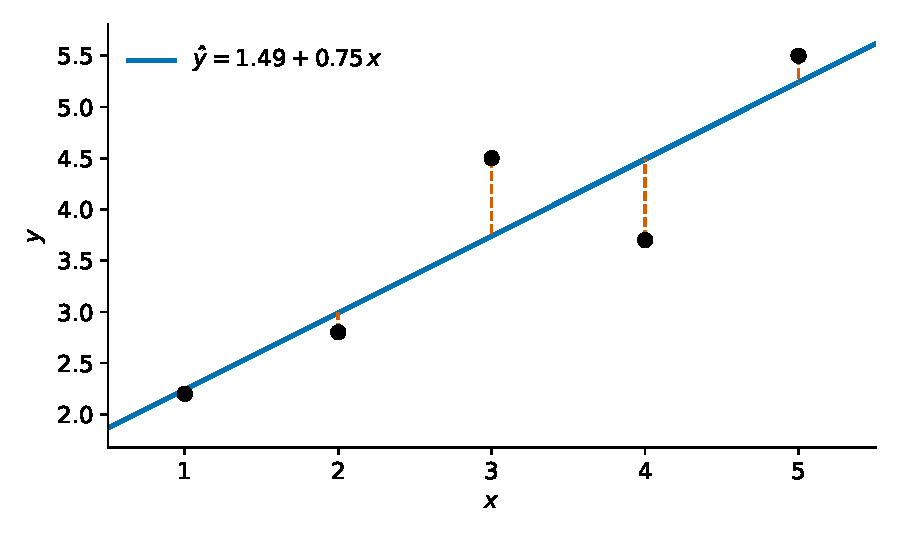
\includegraphics[height=0.6\textheight]{fig_ls_fit.pdf}
\end{center}
\vspace{-6pt}
Residuals $r_i=y_i-\hat y_i$: \; $(-0.04,\ -0.19,\ 0.76,\ -0.79,\ 0.26)$. \quad They sum to zero --- not by
accident (next section).
\end{frame}

\begin{frame}{Rank Deficiency}
If the columns of $\vX$ are linearly dependent (e.g.\ one dummy per category \emph{and} an intercept):
\begin{itemize}
  \item $\vX\T\vX$ is singular; the normal equations have infinitely many solutions.
  \item $\hat\vbeta$ is not identified, but $\hat\vy=\vX\hat\vbeta$ \emph{is} --- every solution gives the
        same fitted values, because they are all the same projection (next section).
  \item Numerically, near-dependence (multicollinearity) makes $(\vX\T\vX)\inv$ huge and $\hat\vbeta$ unstable.
\end{itemize}
\begin{caution}
Never compute $(\vX\T\vX)\inv$ explicitly. Solve the linear system $\vX\T\vX\vbeta=\vX\T\vy$ (Cholesky) or
use the QR / SVD of $\vX$. Lecture 3 (ridge) gives the principled fix for the singular case.
\end{caution}
\end{frame}

% =============================================================================
\sectionframe{The Geometry of Least Squares}
% =============================================================================

\begin{frame}{Least Squares Is a Projection}
Write $\vX=(\vx^{(0)},\vx^{(1)},\dots,\vx^{(p)})$ by columns. Then
\[
\vX\vbeta=\sum_{j=0}^p\beta_j\vx^{(j)}\in\col(\vX),
\]
the subspace of $\R^N$ spanned by the columns. Minimizing $\norm{\vy-\vX\vbeta}^2$ over $\vbeta$ means:
\begin{block}{}
find the point of $\col(\vX)$ closest to $\vy$ --- the \textbf{orthogonal projection} of $\vy$ onto $\col(\vX)$.
\end{block}
\begin{center}
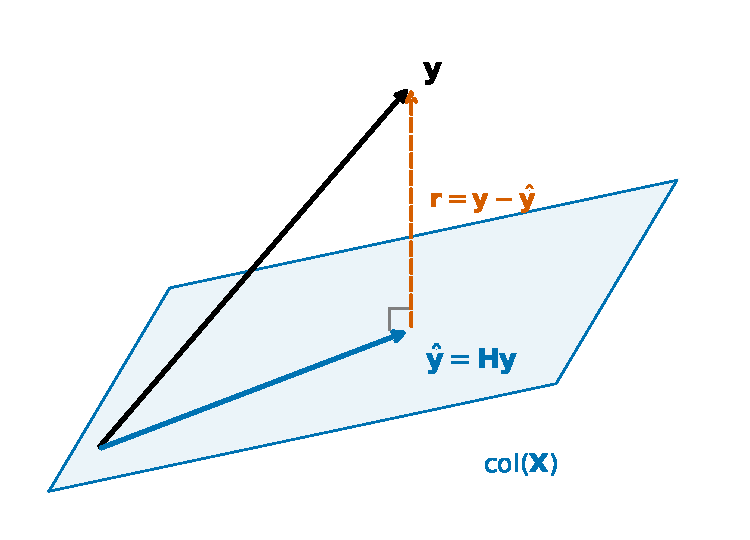
\includegraphics[height=0.38\textheight]{fig_projection.pdf}
\end{center}
\end{frame}

\begin{frame}{The Hat Matrix}
Substituting $\hat\vbeta$ back:
\[
\hat\vy=\vX\hat\vbeta=\vX(\vX\T\vX)\inv\vX\T\vy=\vH\vy,\qquad
\boxed{\vH=\vX(\vX\T\vX)\inv\vX\T}\in\R^{N\times N}.
\]
\begin{claim}{$\vH$ is symmetric and idempotent}
\begin{align*}
\vH\T&=\bigl(\vX(\vX\T\vX)\inv\vX\T\bigr)\T=\vX\bigl((\vX\T\vX)\inv\bigr)\T\vX\T=\vX(\vX\T\vX)\inv\vX\T=\vH,\\
\vH^2&=\vX(\vX\T\vX)\inv\underbrace{\vX\T\vX(\vX\T\vX)\inv}_{=\,\vI}\vX\T=\vX(\vX\T\vX)\inv\vX\T=\vH.
\end{align*}
The first uses $(\vA\vB\vC)\T=\vC\T\vB\T\vA\T$ and that the inverse of a symmetric matrix is symmetric.
\end{claim}
Symmetric + idempotent is exactly the definition of an orthogonal projection matrix.
Projecting twice changes nothing.
\end{frame}

\begin{frame}{Residuals Are Orthogonal to the Fit}
The residual vector is $\vr=\vy-\hat\vy=(\vI-\vH)\vy$.
\begin{derivation}{$\vX\T\vr=\vzero$}
\[
\vX\T\vr=\vX\T\vy-\vX\T\vX\hat\vbeta=\vX\T\vy-\vX\T\vy=\vzero
\qquad\text{(normal equations)}.
\]
\end{derivation}
Consequences:
\begin{itemize}
  \item $\vr$ is orthogonal to every column of $\vX$, hence to all of $\col(\vX)$, hence to $\hat\vy$.
  \item With an intercept, the first column is $\vone$, so $\vone\T\vr=\sum_i r_i=0$: residuals average to zero.
  \item Pythagoras in $\R^N$: \quad $\norm{\vy}^2=\norm{\hat\vy}^2+\norm{\vr}^2$.
\end{itemize}
\begin{keypoint}
$\vI-\vH$ is also a projection --- onto the orthogonal complement $\col(\vX)^\perp$.
\end{keypoint}
\end{frame}

\begin{frame}{Degrees of Freedom}
\begin{claim}{$\tr\vH=p+1$}
Using $\tr(\vA\vB)=\tr(\vB\vA)$,
\[
\tr\vH=\tr\bigl(\vX(\vX\T\vX)\inv\vX\T\bigr)=\tr\bigl((\vX\T\vX)\inv\vX\T\vX\bigr)=\tr\bigl(\vI_{p+1}\bigr)=p+1 .
\]
\end{claim}
\begin{itemize}
  \item A projection matrix has eigenvalues in $\{0,1\}$ (since $\vH^2=\vH\Rightarrow\lambda^2=\lambda$), so its
        trace counts the dimension of the subspace it projects onto.
  \item $\tr\vH$ is the number of parameters --- the \textbf{degrees of freedom} of the fit.
  \item Correspondingly $\tr(\vI-\vH)=N-p-1$: the residual has $N-p-1$ free directions.
        This is where the $N-p-1$ in $\hat\sigma^2$ comes from.
\end{itemize}
\end{frame}

% =============================================================================
\sectionframe{Statistical Properties}
% =============================================================================

\begin{frame}{The Gaussian Model}
So far no probability. Now assume the data were generated by
\[
\vy=\vX\vbeta+\veps,\qquad \veps\sim\Ncal(\vzero,\sigma^2\vI_N),
\]
with $\vX$ fixed and $\vbeta$, $\sigma^2$ unknown. The errors are independent, mean zero, common variance.
\vspace{6pt}

Three questions:
\begin{enumerate}
  \item Is $\hat\vbeta$ centred on $\vbeta$? \hfill (bias)
  \item How much does $\hat\vbeta$ move from sample to sample? \hfill (variance)
  \item Why squared loss and not something else? \hfill (likelihood)
\end{enumerate}
\end{frame}

\begin{frame}{Unbiasedness}
\begin{derivation}{$\E[\hat\vbeta]=\vbeta$}
Substitute the model into the estimator:
\begin{align*}
\hat\vbeta&=(\vX\T\vX)\inv\vX\T\vy=(\vX\T\vX)\inv\vX\T(\vX\vbeta+\veps)\\
&=\underbrace{(\vX\T\vX)\inv\vX\T\vX}_{=\,\vI}\vbeta+(\vX\T\vX)\inv\vX\T\veps
=\vbeta+(\vX\T\vX)\inv\vX\T\veps .
\end{align*}
Taking expectations, with $\vX$ fixed and $\E[\veps]=\vzero$,
\[
\E[\hat\vbeta]=\vbeta+(\vX\T\vX)\inv\vX\T\,\E[\veps]=\vbeta .
\]
\end{derivation}
The estimator equals the truth plus a linear transform of the noise. Everything below follows from that line.
\end{frame}

\begin{frame}{Variance}
\begin{derivation}{$\Var(\hat\vbeta)=\sigma^2(\vX\T\vX)\inv$}
Let $\vA=(\vX\T\vX)\inv\vX\T$ so that $\hat\vbeta-\vbeta=\vA\veps$. For a linear map of a random vector,
$\Var(\vA\veps)=\vA\,\Var(\veps)\,\vA\T$. Hence
\begin{align*}
\Var(\hat\vbeta)&=\vA\,(\sigma^2\vI)\,\vA\T=\sigma^2\,(\vX\T\vX)\inv\vX\T\vX(\vX\T\vX)\inv\\
&=\sigma^2(\vX\T\vX)\inv .
\end{align*}
\end{derivation}
Since $\hat\vbeta$ is an affine function of Gaussian $\veps$, it is Gaussian:
\[
\boxed{\hat\vbeta\sim\Ncal\bigl(\vbeta,\ \sigma^2(\vX\T\vX)\inv\bigr)}
\]
\begin{keypoint}
The variance is driven by $(\vX\T\vX)\inv$. Nearly collinear columns make it large: that is
multicollinearity, stated precisely.
\end{keypoint}
\end{frame}

\begin{frame}{Estimating $\sigma^2$}
\begin{derivation}{$\E\norm{\vr}^2=(N-p-1)\sigma^2$}
$\vr=(\vI-\vH)\vy=(\vI-\vH)(\vX\vbeta+\veps)=(\vI-\vH)\veps$, because $(\vI-\vH)\vX=\vX-\vX=\vzero$.
Then, using $\vI-\vH$ symmetric idempotent and $\E[\veps\T\vM\veps]=\sigma^2\tr\vM$ for fixed $\vM$,
\[
\E\norm{\vr}^2=\E\bigl[\veps\T(\vI-\vH)\T(\vI-\vH)\veps\bigr]=\E\bigl[\veps\T(\vI-\vH)\veps\bigr]
=\sigma^2\tr(\vI-\vH)=\sigma^2(N-p-1).
\]
\end{derivation}
Therefore the \textbf{unbiased} estimator is
\[
\hat\sigma^2=\frac{1}{N-p-1}\sum_{i=1}^N(y_i-\hat y_i)^2,\qquad
(N-p-1)\,\hat\sigma^2\big/\sigma^2\sim\chi^2_{N-p-1},
\]
and $\hat\vbeta$, $\hat\sigma^2$ are independent (they live in orthogonal subspaces, $\col\vX$ and $\col\vX^\perp$).
\end{frame}

\begin{frame}{Where Does Squared Loss Come From?}\small
Under the Gaussian model, $y_i\mid\vx_i\sim\Ncal(\vx_i\T\vbeta,\sigma^2)$, so each observation has density
\[
p(y_i\mid\vx_i;\vbeta,\sigma^2)=\frac{1}{\sqrt{2\pi\sigma^2}}\exp\!\Bigl(-\frac{(y_i-\vx_i\T\vbeta)^2}{2\sigma^2}\Bigr).
\]
\begin{derivation}{Maximum likelihood $=$ least squares}
By independence the likelihood is a product; take logs:
\begin{align*}
\ell(\vbeta,\sigma^2)&=\sum_{i=1}^N\log p(y_i\mid\vx_i)
=-\frac N2\log(2\pi\sigma^2)-\frac{1}{2\sigma^2}\sum_{i=1}^N(y_i-\vx_i\T\vbeta)^2\\
&=-\frac N2\log(2\pi\sigma^2)-\frac{1}{2\sigma^2}\RSS(\vbeta).
\end{align*}
For any fixed $\sigma^2>0$, maximizing $\ell$ over $\vbeta$ is minimizing $\RSS(\vbeta)$.
\end{derivation}
\begin{keypoint}
Squared loss is not a convention. It is the negative log-likelihood of Gaussian noise. Absolute loss
corresponds to Laplace noise; Lecture 2 derives log loss from Bernoulli in the same way.
\end{keypoint}
\end{frame}

\begin{frame}{The MLE of $\sigma^2$ Is Biased}
\begin{derivation}{Maximize $\ell$ over $\sigma^2$ at $\vbeta=\hat\vbeta$}
\[
\frac{\partial\ell}{\partial\sigma^2}=-\frac{N}{2\sigma^2}+\frac{\RSS(\hat\vbeta)}{2\sigma^4}=0
\quad\Longrightarrow\quad
\hat\sigma^2_{\text{MLE}}=\frac{\RSS(\hat\vbeta)}{N}.
\]
\end{derivation}
Compare with the unbiased $\hat\sigma^2=\RSS(\hat\vbeta)/(N-p-1)$:
\[
\E[\hat\sigma^2_{\text{MLE}}]=\frac{N-p-1}{N}\,\sigma^2<\sigma^2 .
\]
The MLE ignores that $p+1$ degrees of freedom were spent fitting $\hat\vbeta$. The discrepancy is
small for $N\gg p$ and the first hint of a theme: \textbf{training error underestimates true error}.
\end{frame}

% =============================================================================
\sectionframe{Gradient Descent}
% =============================================================================

\begin{frame}{Why Not Always Use the Closed Form?}
\begin{itemize}
  \item Solving the normal equations costs $O(Np^2+p^3)$: fine for $p$ in the hundreds, not the millions.
  \item Most losses in this course (log, hinge, exponential) have \emph{no} closed-form minimizer.
  \item Neural networks have none either.
\end{itemize}
\vspace{6pt}
We need a general-purpose optimizer. The simplest one uses only the gradient.
\[
\vtheta^\star=\argmin_{\vtheta\in\R^d}L(\vtheta)
\]
\end{frame}

\begin{frame}{The Update Rule, From Taylor's Theorem}\small
\begin{derivation}{Which small step decreases $L$ the most?}
For a small displacement $\vdelta$,
\[
L(\vtheta+\vdelta)\approx L(\vtheta)+\nabla L(\vtheta)\T\vdelta .
\]
Among all $\vdelta$ with fixed length $\norm{\vdelta}=\eta$, the Cauchy--Schwarz inequality gives
\[
\nabla L(\vtheta)\T\vdelta\ \ge\ -\norm{\nabla L(\vtheta)}\,\norm{\vdelta},
\]
with equality iff $\vdelta$ points along $-\nabla L(\vtheta)$. The steepest descent direction is the
negative gradient.
\end{derivation}
\begin{block}{Gradient descent}
\[
\vtheta^{(t+1)}=\vtheta^{(t)}-\eta\,\nabla L(\vtheta^{(t)}),\qquad \eta>0 \text{ the step size (learning rate)}.
\]
\end{block}
Plugging $\vdelta=-\eta\nabla L$ into the expansion: $L(\vtheta^{(t+1)})\approx L(\vtheta^{(t)})-\eta\norm{\nabla L}^2$.
Each step decreases the loss, \emph{if} $\eta$ is small enough for the approximation to hold.
\end{frame}

\begin{frame}{Gradient Descent for Least Squares}
With $L(\vbeta)=\tfrac{1}{2N}\norm{\vy-\vX\vbeta}^2$ (the $\tfrac1{2N}$ makes the step size scale-free),
\[
\nabla L(\vbeta)=-\frac1N\vX\T(\vy-\vX\vbeta)=-\frac1N\sum_{i=1}^N\bigl(y_i-\vx_i\T\vbeta\bigr)\vx_i .
\]
\begin{block}{Update}
\[
\vbeta^{(t+1)}=\vbeta^{(t)}+\frac{\eta}{N}\sum_{i=1}^N\bigl(y_i-\vx_i\T\vbeta^{(t)}\bigr)\vx_i
\]
\end{block}
Read it: every example pushes $\vbeta$ in the direction of its own input $\vx_i$, weighted by how badly
it is currently predicted. Examples fit exactly contribute nothing.
\end{frame}

\begin{frame}{How Large Can the Step Be?}
Take the simplest case, $L(\theta)=\tfrac12a\theta^2$ with $a>0$, minimum at $\theta^\star=0$.
\begin{derivation}{Exact dynamics}
$\nabla L(\theta)=a\theta$, so
\[
\theta^{(t+1)}=\theta^{(t)}-\eta a\theta^{(t)}=(1-\eta a)\,\theta^{(t)}
\quad\Longrightarrow\quad
\theta^{(t)}=(1-\eta a)^t\,\theta^{(0)}.
\]
The iterates converge iff $\abs{1-\eta a}<1$, i.e.\ \fbox{$0<\eta<2/a$}.
\begin{itemize}
  \item $\eta<1/a$: monotone approach.
  \item $1/a<\eta<2/a$: overshoots and oscillates, but still converges.
  \item $\eta>2/a$: diverges geometrically.
\end{itemize}
\end{derivation}
For a general quadratic $\tfrac12\vtheta\T\vA\vtheta$ the same argument runs along each eigenvector of $\vA$:
the binding constraint is $\eta<2/\lambda_{\max}(\vA)$, and the slowest direction converges at rate
$\abs{1-\eta\lambda_{\min}}$. The ratio $\lambda_{\max}/\lambda_{\min}$ --- the condition number --- governs speed.
\end{frame}

\begin{frame}{Step Size in Pictures}
\begin{center}
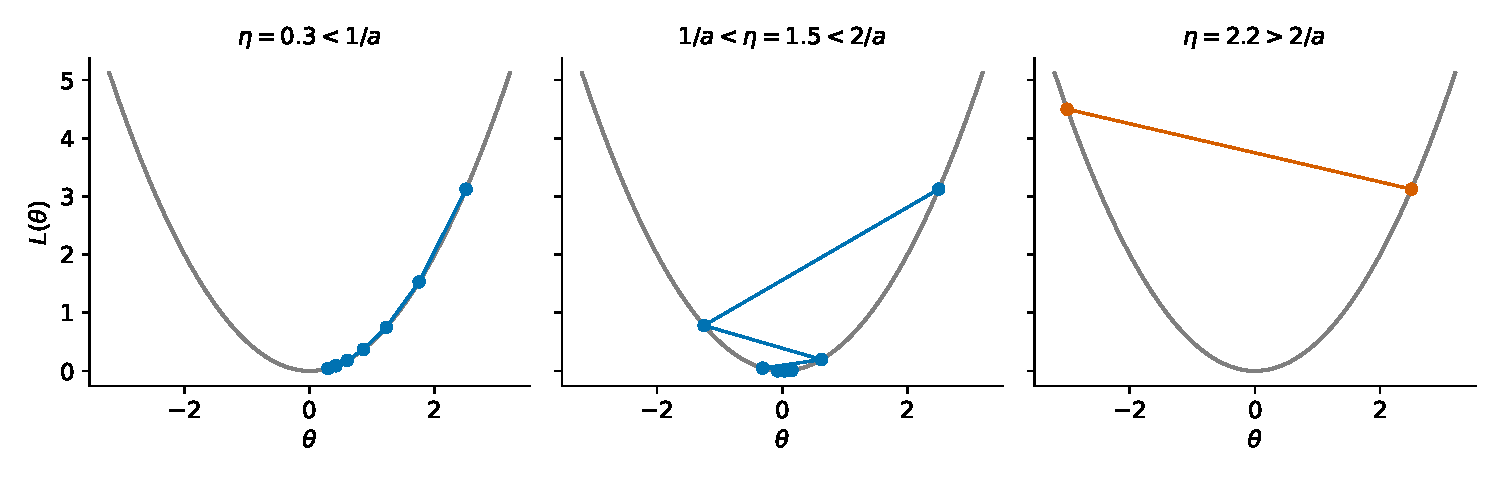
\includegraphics[width=0.85\textwidth]{fig_gd_steps.pdf}
\end{center}
\vspace{-4pt}
Same quadratic, three step sizes. The trajectory on the right is what a too-large $\eta$ looks like in
practice: the loss goes \emph{up}.
\end{frame}

\begin{frame}{Stochastic Gradient Descent}
The full gradient is an average over $N$ terms. Replace it by one term chosen at random:
\[
\vbeta^{(t+1)}=\vbeta^{(t)}+\eta\bigl(y_{i_t}-\vx_{i_t}\T\vbeta^{(t)}\bigr)\vx_{i_t},\qquad i_t\sim\text{Uniform}\{1,\dots,N\}.
\]
\begin{claim}{The stochastic gradient is unbiased}
Let $g_i(\vbeta)=-(y_i-\vx_i\T\vbeta)\vx_i$ be the gradient of the $i$-th term. Then
\[
\E_{i_t}\bigl[g_{i_t}(\vbeta)\bigr]=\sum_{i=1}^N\frac1N\,g_i(\vbeta)=\nabla L(\vbeta).
\]
\end{claim}
So each step moves in the right direction \emph{on average}, at $1/N$ of the cost.
The price is variance: individual steps can point anywhere.
\end{frame}

\begin{frame}{Mini-Batch SGD}
Average over a random subset $\mathcal{B}_t\subset\{1,\dots,N\}$ of size $B$:
\[
\vbeta^{(t+1)}=\vbeta^{(t)}-\frac{\eta}{B}\sum_{i\in\mathcal{B}_t}g_i(\vbeta^{(t)}).
\]
\begin{itemize}
  \item Still unbiased, by the same argument.
  \item Variance of the step shrinks by a factor $B$ (independent draws).
  \item $B=1$ is SGD; $B=N$ is full gradient descent; $B\in[32,256]$ is what everyone uses.
\end{itemize}
\begin{keypoint}
One pass through the data is an \textbf{epoch}. With a constant $\eta$, SGD does not converge to
$\hat\vbeta$; it hovers in a neighbourhood of size $\propto\eta$. Decaying $\eta$ over epochs
(e.g.\ $\eta_t\propto1/t$) is what makes it converge.
\end{keypoint}
\end{frame}

% =============================================================================
\sectionframe{Generalization: Bias and Variance}
% =============================================================================

\begin{frame}{Training Error Is Not the Point}
We minimize $\hat R(f)$, the error on $\Dset$. We care about $R(f)$, the error on new data.
\vspace{6pt}
\begin{center}
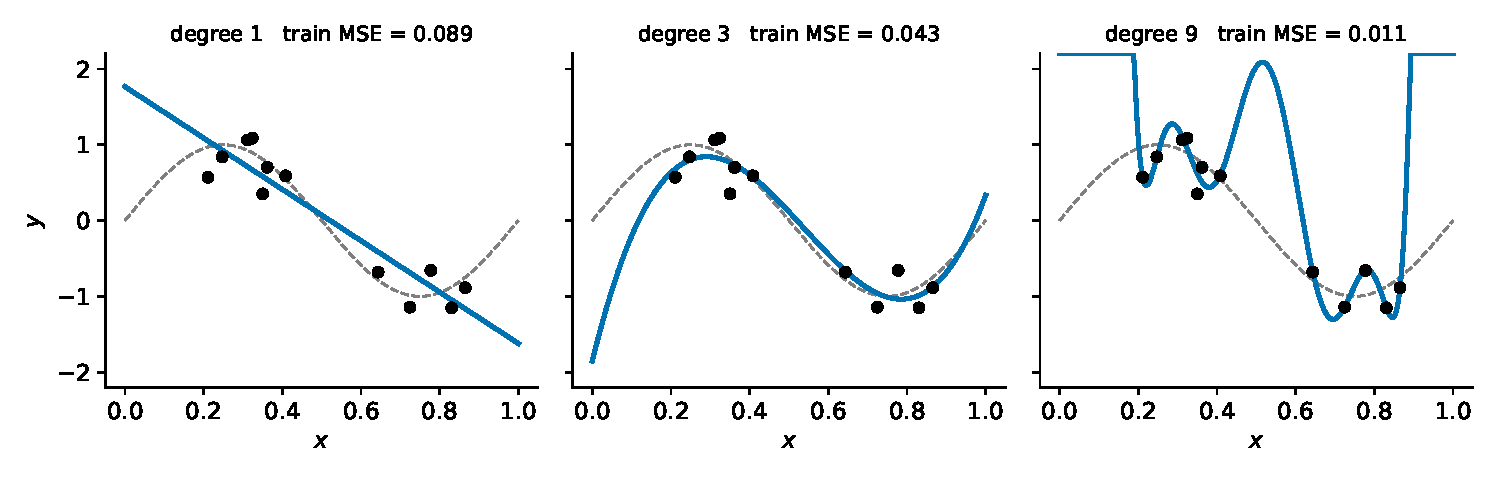
\includegraphics[width=0.75\textwidth]{fig_poly_fits.pdf}
\end{center}
\vspace{-4pt}
Polynomial regression on the same 12 points. Degree 9 has the lowest training error and the worst
predictions. The class $\Hset$ was too rich for the sample.
\end{frame}

\begin{frame}{The Setup for Bias--Variance}
Fix a test input $\vx_0$. The truth is
\[
y_0=f(\vx_0)+\eps_0,\qquad \E[\eps_0]=0,\quad\Var(\eps_0)=\sigma^2 .
\]
Our estimate $\hat f$ was trained on a random sample $\Dset$; it is itself random, with
\[
\bar f(\vx_0)=\E_{\Dset}\bigl[\hat f(\vx_0)\bigr]
\]
its average prediction over all training sets of size $N$. We study the expected test error at $\vx_0$:
\[
\E_{\Dset,\eps_0}\Bigl[\bigl(y_0-\hat f(\vx_0)\bigr)^2\Bigr].
\]
Two sources of randomness, assumed independent: the noise in $y_0$, and the training sample.
\end{frame}

\begin{frame}{The Decomposition}
Write $f=f(\vx_0)$, $\hat f=\hat f(\vx_0)$, $\bar f=\bar f(\vx_0)$.
\begin{derivation}{Split off the noise, then split off the mean}
\begin{align*}
\E\bigl[(y_0-\hat f)^2\bigr]
&=\E\bigl[(f+\eps_0-\hat f)^2\bigr]
=\E\bigl[(f-\hat f)^2\bigr]+\E[\eps_0^2]+2\,\E\bigl[\eps_0(f-\hat f)\bigr]\\
&=\E\bigl[(f-\hat f)^2\bigr]+\sigma^2+2\,\underbrace{\E[\eps_0]}_{0}\,\E[f-\hat f]
&&\text{($\eps_0\perp\Dset$)}\\[6pt]
\E\bigl[(f-\hat f)^2\bigr]
&=\E\bigl[(f-\bar f+\bar f-\hat f)^2\bigr]
=(f-\bar f)^2+\E\bigl[(\bar f-\hat f)^2\bigr]+2(f-\bar f)\underbrace{\E[\bar f-\hat f]}_{0}.
\end{align*}
\end{derivation}
\[
\boxed{\ \E\bigl[(y_0-\hat f)^2\bigr]=\underbrace{\bigl(f-\bar f\bigr)^2}_{\text{Bias}^2}
+\underbrace{\E\bigl[(\hat f-\bar f)^2\bigr]}_{\text{Variance}}
+\underbrace{\sigma^2}_{\text{Noise}}\ }
\]
\end{frame}

\begin{frame}{Reading the Three Terms}
\begin{description}
  \item[Bias$^2$] How far the \emph{average} model is from the truth. Zero if $f\in\Hset$ and the
        estimator is unbiased. Large when $\Hset$ cannot represent $f$.
  \item[Variance] How much $\hat f$ jumps around across training sets. Large when $\Hset$ is rich
        relative to $N$: many members fit the sample, and which one we get depends on the sample.
  \item[Noise] $\sigma^2$. Irreducible. No method can beat it.
\end{description}
\vspace{4pt}
\begin{center}
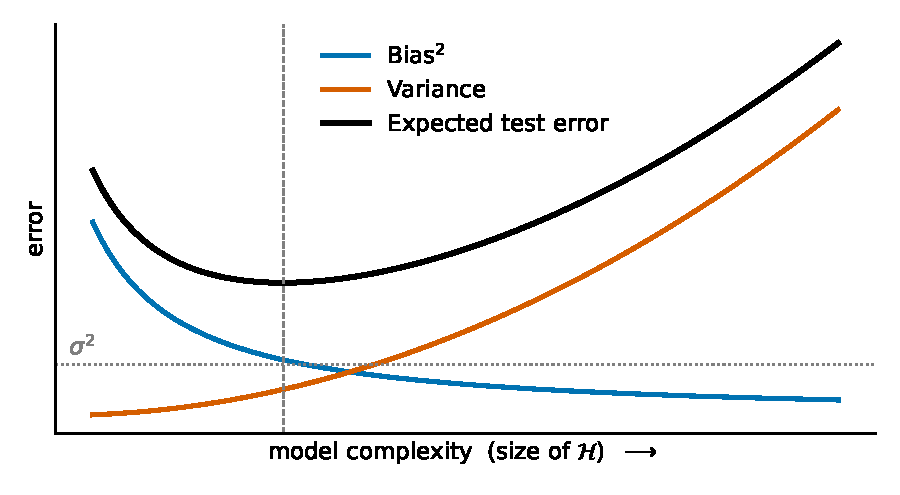
\includegraphics[height=0.5\textheight]{fig_bias_variance.pdf}
\end{center}
\end{frame}

\begin{frame}{Bias--Variance for Least Squares}\footnotesize
When $f(\vx)=\vx\T\vbeta$ is truly linear and $\Dset$ is drawn from the Gaussian model:
\begin{itemize}
  \item $\E[\hat\vbeta]=\vbeta$ (proved above), so $\bar f(\vx_0)=\vx_0\T\vbeta=f(\vx_0)$: \textbf{bias is zero}.
  \item $\Var\bigl(\hat f(\vx_0)\bigr)=\Var(\vx_0\T\hat\vbeta)=\sigma^2\,\vx_0\T(\vX\T\vX)\inv\vx_0$.
\end{itemize}
Averaging the variance over the training inputs $\vx_0\in\{\vx_1,\dots,\vx_N\}$:
\[
\frac1N\sum_{i=1}^N\sigma^2\,\vx_i\T(\vX\T\vX)\inv\vx_i
=\frac{\sigma^2}{N}\tr\bigl(\vX(\vX\T\vX)\inv\vX\T\bigr)
=\frac{\sigma^2}{N}\tr\vH=\sigma^2\,\frac{p+1}{N}.
\]
\begin{keypoint}
Expected test error of least squares $\approx\sigma^2\bigl(1+\tfrac{p+1}{N}\bigr)$. Variance grows
linearly in the number of parameters and shrinks with $N$. Every extra feature costs $\sigma^2/N$ ---
unless it reduces bias by more.
\end{keypoint}
\end{frame}

\begin{frame}{The Trade-Off, and What To Do About It}
Increasing the capacity of $\Hset$ (more features, higher-degree polynomials, deeper trees):
\[
\text{Bias}^2\ \downarrow\qquad\text{Variance}\ \uparrow\qquad\text{Noise unchanged.}
\]
The sum has an interior minimum. Finding it is the practical content of the next lectures:
\begin{itemize}
  \item \textbf{Lecture 3} --- shrink $\hat\vbeta$ toward zero (ridge, lasso): accept a little bias to cut variance.
  \item \textbf{Lecture 4} --- average many high-variance models (bagging): cut variance without adding bias.
  \item \textbf{Lecture 5} --- add low-bias models one at a time (boosting): cut bias under control.
\end{itemize}
\begin{caution}
The decomposition is a statement about \emph{expectations over training sets}. On one sample we never
observe bias or variance separately --- we observe only their sum, and only on held-out data.
\end{caution}
\end{frame}

\begin{frame}{Measuring Generalization: The Protocol}
Since training error is optimistic, hold data out.
\begin{center}
\begin{tabular}{lll}
\toprule
Split & Used for & Touch it how often? \\
\midrule
Training & fitting $\hat\vbeta$ & every iteration \\
Validation & choosing $\Hset$, $\lambda$, $\eta$, stopping time & every candidate \\
Test & reporting the final number & \textbf{once} \\
\bottomrule
\end{tabular}
\end{center}
\vspace{6pt}
\begin{itemize}
  \item Any decision made by looking at a split turns that split into training data.
  \item $K$-fold cross-validation reuses the training set as a rotating validation set; Lab 1 implements it.
  \item The test set is a one-shot instrument. Reuse it and its number stops meaning anything.
\end{itemize}
\end{frame}

% =============================================================================
\sectionframe{Summary}
% =============================================================================

\begin{frame}{What We Proved Today}
\begin{enumerate}
  \item $\nabla_{\vbeta}\RSS=-2\vX\T(\vy-\vX\vbeta)$ and $\nabla^2\RSS=2\vX\T\vX\succeq0$: least squares is convex
        with unique minimizer $\hat\vbeta=(\vX\T\vX)\inv\vX\T\vy$.
  \item $\vH=\vX(\vX\T\vX)\inv\vX\T$ is symmetric, idempotent, $\tr\vH=p+1$: the fit is a projection onto
        $\col(\vX)$ and residuals are orthogonal to it.
  \item Under Gaussian noise, $\hat\vbeta\sim\Ncal(\vbeta,\sigma^2(\vX\T\vX)\inv)$, and least squares is
        maximum likelihood.
  \item Gradient descent is steepest descent from Taylor's theorem; on a quadratic it converges iff $\eta<2/\lambda_{\max}$.
  \item $\E[(y_0-\hat f)^2]=\text{Bias}^2+\text{Variance}+\sigma^2$, and for least squares the variance
        term is $\sigma^2(p+1)/N$.
\end{enumerate}
\end{frame}

\begin{frame}{Next}
\textbf{Lab 1 (Wednesday, Rodrigo)} --- numpy, scikit-learn, the training/validation/test protocol,
$K$-fold cross-validation, and the numerical example of this lecture recomputed from scratch.
\vspace{8pt}

\textbf{Lecture 2 (Friday)} --- the perceptron and its mistake bound; gradient descent
convergence for smooth convex losses; support vector machines and the hinge loss; logistic regression,
its likelihood, and Newton's method.
\vspace{8pt}

\textbf{Reading} --- Hastie, Tibshirani \& Friedman, \emph{The Elements of Statistical Learning},
\S2.1--2.4, \S3.1--3.2, \S7.1--7.3.
\end{frame}

\end{document}
